% rung0-rps-writeup.tex — post-PR writeup for drawmaha-solver PR #1 (rung 0)
\documentclass[11pt]{article}
\usepackage[margin=1.05in]{geometry}
\usepackage{amsmath, amsthm, mathtools}
\usepackage[T1]{fontenc}
\usepackage{newpxtext}
\usepackage{newpxmath}
\usepackage[scaled=0.96]{inconsolata}
\usepackage{microtype}
\usepackage{graphicx}
\usepackage{booktabs}
\usepackage{array}
\usepackage{xcolor}
\usepackage[most]{tcolorbox}
\usepackage{titlesec}
\usepackage{enumitem}
\usepackage{caption}
\usepackage{fvextra}
\usepackage{float}
\usepackage{needspace}
\tcbuselibrary{breakable, skins}
\usepackage[colorlinks=true, allcolors=blueaccentlink]{hyperref}

\definecolor{blueaccent}{HTML}{134A6B}
\definecolor{blueaccentlink}{HTML}{1A5E88}
\definecolor{teal}{HTML}{2C6E63}
\definecolor{rust}{HTML}{B4623C}
\definecolor{indigo}{HTML}{574B93}
\definecolor{ink}{HTML}{1A1A1A}
\definecolor{softgray}{HTML}{667079}
\definecolor{rulegray}{HTML}{C9CED3}
\definecolor{goalBg}{HTML}{E3EDF4}\definecolor{goalRule}{HTML}{1A5E88}
\definecolor{intBg}{HTML}{DCEAF3}\definecolor{intRule}{HTML}{134A6B}
\definecolor{decBg}{HTML}{E5E1F1}\definecolor{decRule}{HTML}{574B93}
\definecolor{exBg}{HTML}{DBEDE7}\definecolor{exRule}{HTML}{2C6E63}
\definecolor{gotBg}{HTML}{F6E4D9}\definecolor{gotRule}{HTML}{B4623C}
\definecolor{codeBg}{HTML}{EEF3F7}\definecolor{codeRule}{HTML}{7FA6C4}
\color{ink}

\titleformat{\section}[hang]{\Large\bfseries\color{blueaccent}}{\textcolor{rust}{\thesection}}{0.6em}{}[%
  \nobreak{\vspace{-4pt}\color{blueaccent!35}\titlerule[1.2pt]}\nobreak]
\titlespacing*{\section}{0pt}{1.4em}{0.6em}
\titleformat{\subsection}[hang]{\large\bfseries\color{blueaccent!92}}{\textcolor{rust}{\thesubsection}}{0.6em}{}

\captionsetup{font=small, labelfont={bf,color=blueaccent}, labelsep=period,
  textfont={color=softgray}, width=0.94\linewidth}

\newtcolorbox{calloutbox}[3]{
  enhanced, breakable, frame hidden, sharp corners, arc=0pt,
  colback=#1, boxrule=0pt, borderline west={4pt}{0pt}{#2},
  left=14pt, right=12pt, top=8pt, bottom=8pt, before skip=10pt, after skip=10pt,
  fonttitle=\bfseries\footnotesize, coltitle=#2,
  attach boxed title to top left={xshift=14pt, yshift=-2pt},
  boxed title style={frame hidden, colback=white, arc=1pt, left=3pt, right=3pt},
  title=\textsc{#3}
}
\newenvironment{goal}{\begin{calloutbox}{goalBg}{goalRule}{Outcome}}{\end{calloutbox}}
\newenvironment{intuition}{\begin{calloutbox}{intBg}{intRule}{Takeaway}}{\end{calloutbox}}
\newenvironment{decision}{\begin{calloutbox}{decBg}{decRule}{Decision}}{\end{calloutbox}}
\newenvironment{example}{\begin{calloutbox}{exBg}{exRule}{Example}}{\end{calloutbox}}
\newenvironment{gotcha}{\begin{calloutbox}{gotBg}{gotRule}{Risk}}{\end{calloutbox}}

\newtcbox{\chip}{on line, boxrule=0pt, boxsep=0pt, left=3pt, right=3pt,
  top=1pt, bottom=1pt, arc=2.5pt, colback=blueaccent!9, coltext=blueaccent!85!black,
  fontupper=\ttfamily\small}

\newtcolorbox{codebox}{
  breakable, enhanced, sharp corners, boxrule=0pt, frame hidden,
  colback=codeBg, borderline west={3pt}{0pt}{codeRule},
  left=10pt, right=8pt, top=6pt, bottom=6pt, before skip=9pt, after skip=9pt,
}

\newcommand{\source}[1]{{\small\textcolor{softgray}{[\,source: \texttt{#1}\,]}}}

\title{\vspace{-1.2cm}{\color{blueaccent}\textbf{Rung 0: RPS Regret Matching --- Post-PR Writeup}}\\[2pt]
  \large\normalfont\color{softgray} drawmaha-solver PR \#1: the learning rule, proven on the smallest game}
\author{\normalsize\color{softgray} What actually shipped, and how}
\date{\normalsize\small\color{softgray} Companion artifact: \texttt{rung0-rps-writeup.md}. Synthesized by Claude from the merged diff and local test runs.}

\emergencystretch=2.5em

\begin{document}
\maketitle
\vspace{-0.7cm}

% =================== 1. Outcome & decision summary ==========================
\section{Outcome \& decision summary}

\noindent The drawmaha-solver project is building a neural poker solver for
heads-up Drawmaha (a split-pot draw/Omaha hybrid with no existing solver),
developed as a ladder of five rungs: each rung adds one layer of complexity and
is verified against a known answer before climbing. This PR ships \textbf{rung
0} --- the \emph{regret-matching} learning rule, the algorithm at the heart of
every later rung, implemented on rock-paper-scissors, the smallest game with a
known mixed-strategy equilibrium. It also establishes the Python package, test
harness, and figure pipeline every later rung builds on.

\begin{goal}
\textbf{The learner provably works} --- its average strategy converges to the
known Nash equilibrium (a best-responding adversary wins only 0.0009
chips/round off it after 100k iterations), and against a biased opponent it
converges to the exploiting counter. \textbf{The ask: approve and merge PR \#1
into \texttt{main}.} No migrations, no deploys, no ordering conditions. All 38
tests pass locally; the repository has no CI yet (the one gray tile in \S4;
follow-up in \S6). Verdict: \textbf{merge-ready}.
\end{goal}

\begin{table}[H]
\centering\small
\caption{The PR, in plain words.}
\renewcommand{\arraystretch}{1.25}
\begin{tabular}{@{}lp{9.9cm}r@{}}
\toprule
PR & What it does & Size \\
\midrule
\#1 & Adds the rung-0 package: the RPS rules, the regret-matching learner, a
      match runner with human/fixed/learner players, a convergence analysis
      that certifies the learner finds the Nash equilibrium (four committed
      figures), and a terminal game to play against it. & 18 files, $+$1,310 \\
\bottomrule
\end{tabular}
\end{table}

% =================== 2. The algorithm and the as-built map ==================
\section{The algorithm, and the as-built map}

\noindent Everything in this PR lives in one Python package plus its tests; the
map below shows the two ways in and what they share. Four terms carry the whole
document. \textbf{Regret}: after a round, for each action you \emph{could} have
played, how much better it would have scored than what you did.
\textbf{Regret matching}: the learning rule --- next round, play each action
with probability proportional to its accumulated \emph{positive} regret
(uniform if none is positive). \textbf{Current vs.\ average strategy}: the
current strategy cycles forever and never settles; the theorem is that the
\emph{running average} of all strategies played converges to the Nash
equilibrium --- the average is the product. \textbf{Exploitability}: the score
--- how much a best-responding adversary who knows your strategy wins per round
against it; exactly 0 at the Nash equilibrium, and the project's evaluation
currency all the way up the ladder.

\begin{example}
The ledger after one round, starting uniform $(\tfrac13,\tfrac13,\tfrac13)$:
the opponent shows paper, so the utility of each of our actions is (rock $-1$,
paper $0$, scissors $+1$). Our strategy's expected utility is $0$, so the
regret increments are the utilities themselves: $(-1, 0, +1)$. Only scissors
has positive regret, so the next round plays scissors with probability 1 ---
and the average strategy has banked one uniform round.
\end{example}

\begin{figure}[H]
\centering
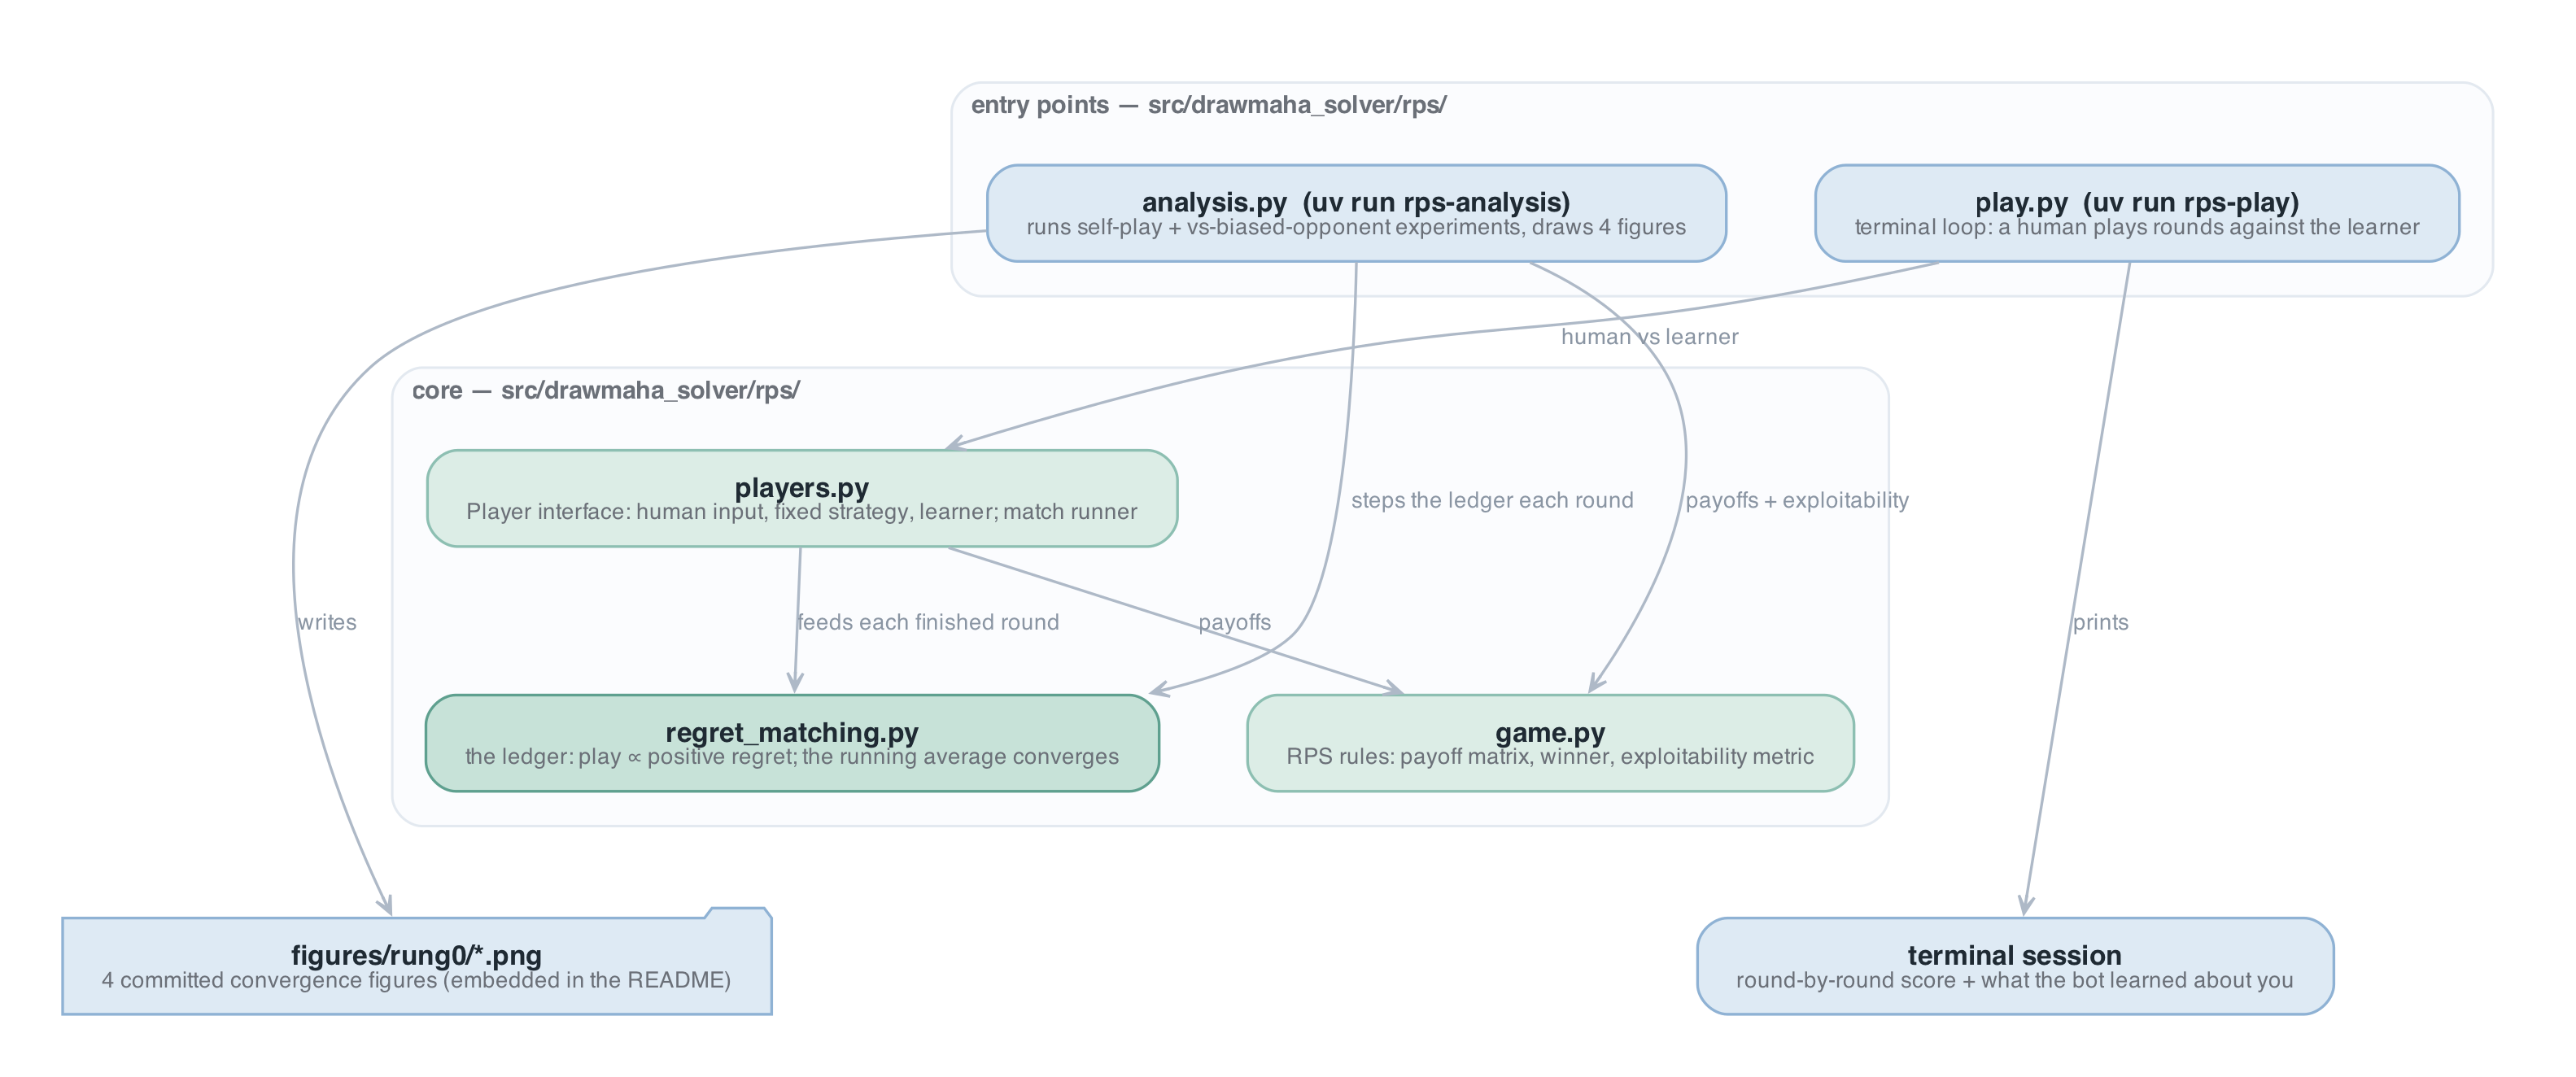
\includegraphics[width=0.98\linewidth]{diagrams/as_built_architecture.png}
\caption{The package as merged. Green = new code (everything is new at rung 0);
blue = entry points and outputs. Two entry points branch into a shared core:
the analysis CLI drives the ledger directly, the play CLI goes through the
player layer, and both converge on the ledger and the rules.}
\label{fig:asbuilt}
\end{figure}

% =================== 3. How it works ========================================
\needspace{0.30\textheight}
\section{How it works}

\noindent One PR, five modules, walked in the diagram's causal order. Per
file: what it is, then the facts that matter.

\medskip
\noindent\textbf{\texttt{game.py}} --- the rules of RPS, and the measuring stick.
\begin{itemize}[leftmargin=*, nosep]
  \item the payoff matrix (\chip{PAYOFF[a, b]} = row player's chips) is the
        single source of truth; zero-sum and antisymmetric by construction
        \source{src/drawmaha\_solver/rps/game.py:32}
  \item \chip{winner(a, b)} derives win/loss/tie from the matrix, never from a
        second rules table \source{game.py:44}
  \item \chip{best\_response\_value(strategy)} is the exploitability metric ---
        the project's first evaluation instrument \source{game.py:61}
  \item actions are an \chip{IntEnum} so they index payoff matrices and
        strategy vectors directly \source{game.py:21}
\end{itemize}

\medskip
\noindent\textbf{\texttt{regret\_matching.py}} --- the learner: one ledger,
$\sim$40 lines, the heart of the project.
\begin{itemize}[leftmargin=*, nosep]
  \item \chip{strategy()} normalizes positive accumulated regrets;
        all-negative regrets fall back to uniform
        \source{regret\_matching.py:36}
  \item \chip{update(utilities)} accumulates regret against the strategy's
        \emph{expected} utility and banks the strategy into the running
        average \source{regret\_matching.py:51}
  \item \chip{average\_strategy()} returns the running average --- the object
        that converges \source{regret\_matching.py:44}
  \item a one-action ledger is rejected loudly rather than degenerating
        silently \source{regret\_matching.py:31}
\end{itemize}

\begin{codebox}
\begin{Verbatim}[fontsize=\small, breaklines, breakanywhere]
def update(self, utilities: np.ndarray) -> None:
    current = self.strategy()
    self.strategy_sum += current
    self.cumulative_regret += utilities - current @ utilities
\end{Verbatim}
\end{codebox}

\begin{decision}
The ledger measures regret against the strategy's expected utility
$u - \langle\sigma, u\rangle$, not against the sampled action (the textbook
RPS-trainer variant) --- \emph{because} that is exactly the counterfactual-regret
form CFR uses at every information set, so rung 1 changes nothing about the
update rule; and it is lower-variance: final exploitability 0.00091 chips/round
vs 0.00443 for the sampled form on the same budget. Don't ``simplify'' it back.
\end{decision}

\medskip
\noindent\textbf{\texttt{players.py}} --- the glue: who plays, and how rounds flow.
\begin{itemize}[leftmargin=*, nosep]
  \item \chip{Player} is a two-method interface: \chip{act(rng)} and
        \chip{observe(own, opp)} \source{players.py:19}
  \item \chip{RegretMatchingPlayer.observe} feeds the ledger
        \chip{PAYOFF[:, opp]} --- the utility of every action against the
        opponent's revealed move \source{players.py:53}
  \item \chip{FixedStrategyPlayer} rejects any input that is not a probability
        distribution \source{players.py:37}
  \item \chip{play\_match(p0, p1, *, n\_rounds, rng)} runs rounds, shows both
        players the result, returns player 0's payoffs \source{players.py:85}
\end{itemize}

\medskip
\noindent\textbf{\texttt{analysis.py}} --- the certification: experiments plus
the four committed figures.
\begin{itemize}[leftmargin=*, nosep]
  \item \chip{run\_self\_play} records, per iteration, the current strategy,
        the running average, and the average's exploitability
        \source{analysis.py:98}
  \item \chip{run\_vs\_fixed} pits the learner against a fixed 50\%-rock
        opponent \source{analysis.py:121}
  \item results travel as frozen dataclasses, not loose dicts
        \source{analysis.py:49}
  \item four figures (average-strategy convergence, current-vs-average cycling,
        log--log exploitability decay, best-response learning) write to
        \texttt{figures/rung0/} \source{analysis.py:139}
\end{itemize}

\medskip
\noindent\textbf{\texttt{play.py}} --- the demo: \chip{uv run rps-play} is a
terminal loop against the learner; on quit it prints the bot's learned average
strategy --- against a habit-prone human it visibly drifts toward the counter
\source{play.py:10}.

% =================== 4. Test results ========================================
\needspace{0.5\textheight}
\section{Test results}

\noindent All 38 tests pass, run locally on this branch (\texttt{uv run
pytest}, 1.4\,s). Every count below is paired with what it proves; the one
gray tile is the \emph{absence} of CI, not a failing check.

\begin{figure}[H]
\centering
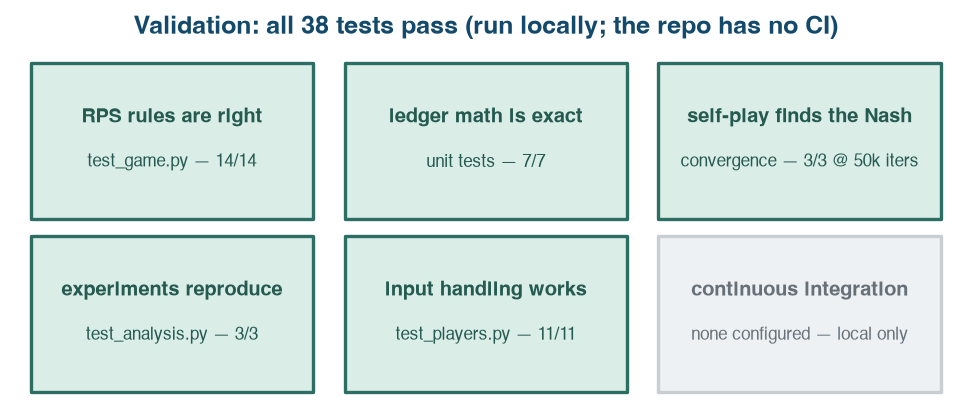
\includegraphics[width=0.9\linewidth]{figures/validation_grid.png}
\caption{Teal = passed locally; gray = not verifiable (the repository has no
CI). Tile titles say what passing proves.}
\label{fig:val}
\end{figure}

\begin{itemize}[leftmargin=*, nosep]
  \item \textbf{14 rules tests} prove the game itself is right: all 9
        action-pair outcomes pinned individually, the payoff matrix verified
        zero-sum, and the exploitability metric anchored at both extremes
        (uniform $\to$ 0, pure rock $\to$ 1) plus a hand-computed midpoint.
  \item \textbf{7 ledger unit tests} prove the math is exact, not just
        plausible: hand-computed regret increments for the expected-utility
        update, the positive-regret normalization, the uniform fallback, and
        the average-strategy arithmetic.
  \item \textbf{3 convergence tests} prove the theorem shows up in practice:
        50k-iteration self-play lands within 0.02 of the uniform Nash with
        exploitability $<$ 0.02 for \emph{both} players; against a 50\%-rock
        opponent the average goes $>$ 90\% paper and realized winnings beat
        $+$0.1/round; identical seeds reproduce identical matches.
  \item \textbf{3 analysis tests} prove the certification pipeline reproduces:
        trajectory shapes, exploitability falling over time, and all four
        figure files actually written.
  \item \textbf{11 input-handling tests} prove the boundary is defended:
        non-distributions rejected, r/p/s and full words parsed, garbage
        reprompted, quit raised cleanly.
\end{itemize}

\medskip
\noindent Headline numbers from the committed 100k-iteration run: self-play
average strategy $(0.334, 0.333, 0.333)$, exploitable for \textbf{0.00091
chips/round}; against 50\% rock the learner's average is 99.9\% paper earning
\textbf{$+$0.237/round} (the theoretical best response earns $+$0.25).

\begin{figure}[H]
\centering

\includegraphics[width=0.82\linewidth]{figures/self_play_average_strategy.png}
\caption{What convergence actually looks like: each action's average
probability (log-scale iterations) swinging early, then locking onto the 1/3
line. The other three committed figures show the current strategy cycling
forever, the $1/\sqrt{T}$ exploitability decay, and the best-response
convergence.}
\label{fig:conv}
\end{figure}

% =================== 5. Edge cases & handling ===============================
\needspace{0.22\textheight}
\section{Edge cases \& handling}

\noindent The boundaries the change has to survive, each with its current
status and where it is handled.

\begin{table}[H]
\centering\small
\caption{Edge cases \& handling. Paths are under \texttt{src/drawmaha\_solver/rps/}.}
\renewcommand{\arraystretch}{1.25}
\begin{tabular}{@{}p{7.2cm}p{2.6cm}p{3.6cm}@{}}
\toprule
Case & Status & Where handled \\
\midrule
One-action ledger (degenerate game) & handled --- raises & \texttt{regret\_matching.py:31} \\
All regrets negative (no positive signal) & handled --- uniform & \texttt{regret\_matching.py:40} \\
Player given a non-distribution strategy & handled --- raises & \texttt{players.py:37} \\
Garbage terminal input & handled --- reprompts & \texttt{players.py:79} \\
Quit before playing any round & handled --- no summary & \texttt{play.py:38} \\
Analysis run shorter than the 5{,}000-iteration plot window & handled --- clamps & \texttt{analysis.py:156} \\
\chip{update()} given a wrong-length utilities vector & \emph{known gap} & see below \\
\bottomrule
\end{tabular}
\end{table}

\noindent The known gap: numpy raises on the length mismatch, but only
\emph{after} the strategy was banked into the average --- the ledger is left
half-updated \source{regret\_matching.py:51}. Accepted at rung 0 (the only
callers are in-repo and tested); harden the boundary when the API grows
callers at rung 1.

% =================== 6. Risks & follow-ups ==================================
\needspace{0.22\textheight}
\section{Risks \& follow-ups}

\noindent Only what is still true after merge.

\begin{gotcha}
\textbf{Nothing guards \texttt{main}:} the repository has no CI, so these 38
tests run only when someone runs them --- a future PR could break the ladder's
foundation silently $\to$ add a GitHub Actions \texttt{uv run pytest} workflow
before rung 1 lands.
\end{gotcha}

\begin{itemize}[leftmargin=*, nosep]
  \item \textbf{Convergence tests are seed-pinned} --- a numpy RNG behavior
        change could flip a threshold $\to$ \texttt{uv.lock} is committed and
        pins numpy; keep it that way.
  \item \textbf{README numbers and figures regenerate only manually} --- if the
        ledger changes, \texttt{uv run rps-analysis} must be re-run or the
        committed figures drift from the code.
  \item \textbf{The interactive play loop has no test of its own} --- input
        \emph{parsing} is tested (11 tests); the \chip{play.main()} round loop
        is exercised only by hand.
  \item \textbf{Deferred (by design):} rung 1 --- tabular CFR on Kuhn poker
        against the known exact equilibrium --- is next; nothing in this PR
        blocks its shape beyond the update rule deliberately matching CFR's.
\end{itemize}

% =================== 7. Validation & merge-readiness gate ===================
\needspace{0.30\textheight}
\section{Validation \& merge-readiness gate}

\noindent The final verdict, echoing \S1's ask.

\begin{table}[H]
\centering\small
\caption{Merge-readiness gate.}
\renewcommand{\arraystretch}{1.25}
\begin{tabular}{@{}p{4.0cm}p{3.4cm}p{5.6cm}@{}}
\toprule
Gate & Status & Note \\
\midrule
Branch / commits & \texttt{alec/rung0-rps} & \texttt{983066b}, \texttt{623b96b} --- \href{https://github.com/AlecROndo/drawmaha-solver/pull/1}{PR \#1} \\
Merge conflicts  & none & \texttt{mergeable: MERGEABLE}, state \texttt{CLEAN} \\
CI / checks      & n/a & no CI configured on this repository (\S6) \\
Tests (local)    & 38/38 pass & \texttt{uv run pytest}, verified on the PR tip \\
Review           & 0 open & no human review yet; single-author repository \\
Migrations / deploy & none & pure library + CLI code \\
\bottomrule
\end{tabular}
\end{table}

\noindent\textbf{Bottom line: safe to merge as-is;} the only outstanding items
are the no-CI follow-up and the one known gap, both accepted for rung 0.

\end{document}
